\documentclass[compress]{beamer}
%,hyperref={pdfpagelabels=false}

\usepackage[ngerman,english]{babel}
\usepackage[T1]{fontenc}
\usepackage[latin1]{inputenc}
\usepackage{amsmath}
\usepackage{amsthm}
\usepackage{amsfonts}
\usepackage{helvet}
\usepackage{url}
\usepackage{listings}
\usepackage{xcolor}
\usepackage{color}
\usepackage{xspace} % Abstand hinter Variablennamen
\usepackage{fix-cm}
\usepackage{graphicx}
\usepackage{subfigure}
%\usepackage[square, sort, numbers, authoryear]{natbib}

\usepackage{beamerthemeLEA2}

%\bibliographystyle{plainnat}

\newcommand{\N}       {\mathbb{N}}          % natürliche Zahlen
\newcommand{\Z}       {\mathbb{Z}}          % ganze Zahlen
\newcommand{\R}       {\mathbb{R}}          % reelle Zahlen
\newcommand{\Prob}    {\mathrm{P}}          % Wahrscheinlichkeit
\newcommand{\inter}   {\cap}                % Schnittmenge
\newcommand{\union}   {\cup}                % Vereinigung
\newcommand{\Oh}      {O}                   % O-Notation (Landau-Symbole)
\newcommand{\mycite}[1]{\textcolor{tumgreen}{[#1]}} 

\newenvironment{changemargin}[2]{% 
  \begin{list}{}{%
    \setlength{\topsep}{0pt}%
    \setlength{\leftmargin}{#1}%
    \setlength{\rightmargin}{#2}%
    \setlength{\listparindent}{\parindent}%
    \setlength{\itemindent}{\parindent}%
    \setlength{\parsep}{\parskip}%
  }%
  \item[]}{\end{list}}
  
\definecolor{light-gray}{gray}{0.95}
\definecolor{middle-gray}{gray}{0.5}
  
\lstset{basicstyle=\footnotesize\ttfamily,breaklines=true}
\lstset{columns=fullflexible}
\lstset{framextopmargin=20pt}
\lstset{backgroundcolor=\color{white}}
\lstset{escapeinside={<@}{@>}}

\title{A Flexible Tool for Shape Analysis}
\subtitle{IDP Presentation}
\author{\href{emanuel.laude@in.tum.de}{Emanuel Laude}\\ \href{laehner@in.tum.de}{Zorah L\"ahner} } 
%\date{\today}
\date{January 16, 2015}
\institute{Technische Universit\"at M\"unchen}

% Inhaltsverzeichnis zu Begin von jedem Abschnitt einblenden?
%\AtBeginSection[]{
%  \begin{frame}
%    \frametitle{Outline}
%    \tableofcontents[currentsection]
%  \end{frame}
%}

\begin{document}

\begin{frame}
  \titlepage
\end{frame}

% Inhaltsverzeichnis
\begin{frame}
  \frametitle{Outline}
  \tableofcontents
\end{frame}

\section{Demo Time}

\begin{frame}
	\frametitle{Introduction}
	
	\bf{Demo Time}
	
\end{frame}

\section{Class Overview}

\begin{frame}
  \frametitle{Class Diagram: View}
  \begin{figure}[h]
	\centering
	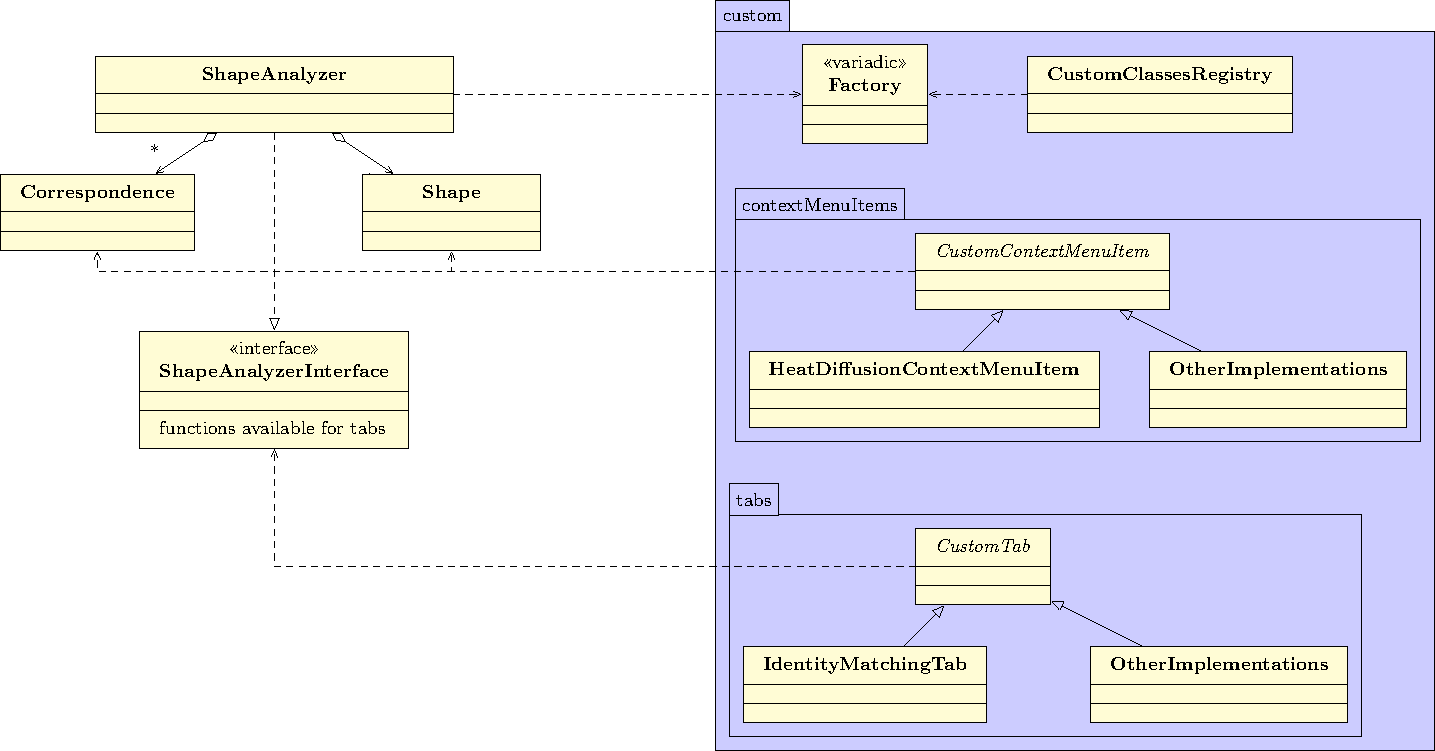
\includegraphics[width=\textwidth]{diagram.pdf}
\end{figure}
\end{frame}

\begin{frame}
  \frametitle{Class Diagram: Domain}
  \begin{figure}[h]
	\centering
	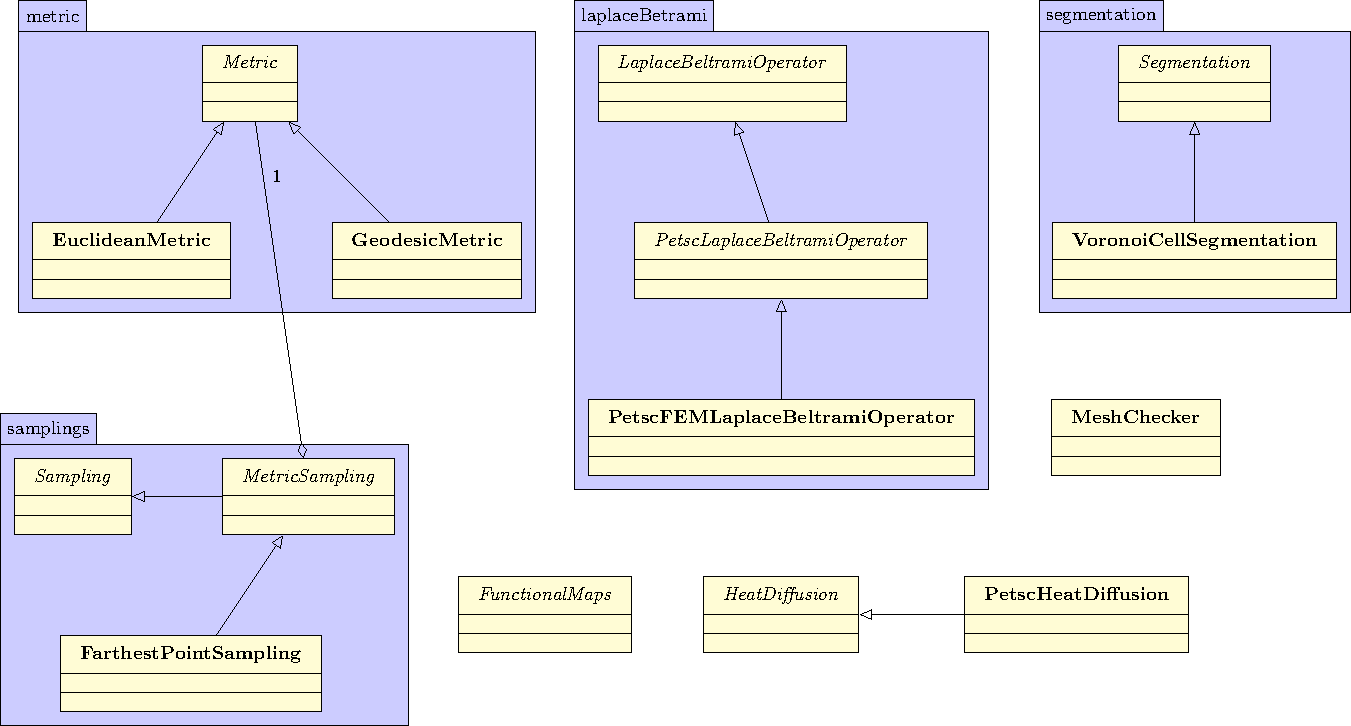
\includegraphics[width=\textwidth]{diagram2.pdf}
\end{figure}
\end{frame}

\section{Customs}

\begin{frame}[c]
  \frametitle{Customs}
  \begin{center}
  
  \huge CustomContextMenuItem 
  
  \vspace{1em}
  
  or 
  
  \vspace{1em}
  
  CustomTab?
  \end{center}
\end{frame}

\begin{frame}[fragile]
  \frametitle{Example: VoronoiCellsContextMenuItem}
  
\begin{lstlisting}[language=C++, keywordstyle=\color{blue},
                stringstyle=\color{red},
                commentstyle=\color{green}, numbers=none]
<@\textcolor{middle-gray}{template<class T = Metric>}@>
class VoronoiCellsContextMenuItem : public CustomContextMenuItem {
<@\textcolor{middle-gray}{public:}@>
	<@\textcolor{middle-gray}{VoronoiCellsContextMenuItem<T>}@>
	<@\textcolor{middle-gray}{(shared\_ptr<Shape> shape, ShapeAnalyzerInterface* shapeAnalyzer)}@>
	 <@\textcolor{middle-gray}{: CustomContextMenuItem(shape, shapeAnalyzer) \{ \}}@>
    
    <@\textcolor{middle-gray}{virtual void onClick(vtkIdType pointId, vtkIdType faceId, QWidget* parent) \{}@>
        <@\textcolor{middle-gray}{(...)    \}}@>
<@\textcolor{middle-gray}{\};}@>
\end{lstlisting}
  
\end{frame}

\begin{frame}[fragile]
  \frametitle{Example: VoronoiCellsContextMenuItem}
  
\begin{lstlisting}[language=C++, keywordstyle=\color{blue},
                stringstyle=\color{red},
                commentstyle=\color{green}, numbers=none]
template<class T = Metric>
<@\textcolor{middle-gray}{class VoronoiCellsContextMenuItem : public CustomContextMenuItem \{}@>
<@\textcolor{middle-gray}{public:}@>
	<@\textcolor{middle-gray}{VoronoiCellsContextMenuItem<T>}@>
	<@\textcolor{middle-gray}{(shared\_ptr<Shape> shape, ShapeAnalyzerInterface* shapeAnalyzer)}@>
	 <@\textcolor{middle-gray}{: CustomContextMenuItem(shape, shapeAnalyzer) \{ \}}@>
    
    <@\textcolor{middle-gray}{virtual void onClick(vtkIdType pointId, vtkIdType faceId, QWidget* parent) \{}@>
        <@\textcolor{middle-gray}{(...)    \}}@>
<@\textcolor{middle-gray}{\};}@>
\end{lstlisting}
  
\end{frame}

\begin{frame}[fragile]
  \frametitle{Example: VoronoiCellsContextMenuItem}
  
\begin{lstlisting}[language=C++, keywordstyle=\color{blue},
                stringstyle=\color{red},
                commentstyle=\color{green}, numbers=none]
<@\textcolor{middle-gray}{template<class T = Metric>}@>
<@\textcolor{middle-gray}{class VoronoiCellsContextMenuItem : public CustomContextMenuItem \{}@>
<@\textcolor{middle-gray}{public:}@>
	VoronoiCellsContextMenuItem<T>
	 (shared_ptr<Shape> shape, ShapeAnalyzerInterface* shapeAnalyzer)
	 	: CustomContextMenuItem(shape, shapeAnalyzer) { }
    
    <@\textcolor{middle-gray}{virtual void onClick(vtkIdType pointId, vtkIdType faceId, QWidget* parent) \{}@>
        <@\textcolor{middle-gray}{(...)    \}}@>
<@\textcolor{middle-gray}{\};}@>
\end{lstlisting}
  
\end{frame}

\begin{frame}[fragile]
  \frametitle{Example: VoronoiCellsContextMenuItem}
  
\begin{lstlisting}[language=C++, keywordstyle=\color{blue},
                stringstyle=\color{red},
                commentstyle=\color{green}, numbers=none]
<@\textcolor{middle-gray}{template<class T = Metric>}@>
<@\textcolor{middle-gray}{class VoronoiCellsContextMenuItem : public CustomContextMenuItem \{}@>
<@\textcolor{middle-gray}{public:}@>
	<@\textcolor{middle-gray}{VoronoiCellsContextMenuItem<T>}@>
	<@\textcolor{middle-gray}{(shared\_ptr<Shape> shape, ShapeAnalyzerInterface* shapeAnalyzer)}@>
	 <@\textcolor{middle-gray}{: CustomContextMenuItem(shape, shapeAnalyzer) \{ \}}@>
    
    virtual void onClick(vtkIdType pointId, vtkIdType faceId, QWidget* parent) {
        (...)    }
<@\textcolor{middle-gray}{\};}@>
\end{lstlisting}
  
\end{frame}


\begin{frame}[fragile]
  \frametitle{Example: VoronoiCellsContextMenuItem}
  
\begin{lstlisting}[language=C++, keywordstyle=\color{blue},
                stringstyle=\color{red},
                commentstyle=\color{green}, numbers=none]
<@\textcolor{middle-gray}{virtual void onClick(...) \{}@>
    <@\textcolor{middle-gray}{bool ok;}@>
    vtkIdType source = QInputDialog::getInt(...);
    <@\textcolor{middle-gray}{if (!ok) \{ return; \}}@>
    <@\textcolor{middle-gray}{(...)}@>
    <@\textcolor{middle-gray}{if(ok) \{}@>
        <@\textcolor{middle-gray}{try \{}@>
            <@\textcolor{middle-gray}{auto m = make\_shared<T>(shape\_);}@>
            <@\textcolor{middle-gray}{auto fps = make\_shared<FarthestPointSampling>(shape\_, m, source, numberOfSegments);}@>
            <@\textcolor{middle-gray}{VoronoiCellSegmentation segmentation(shape\_, m, fps);}@>
            <@\textcolor{middle-gray}{shape\_->setColoring(segmentation.getSegments(), }@>
            	<@\textcolor{middle-gray}{Shape::Coloring::Type::PointSegmentation);}@>
        <@\textcolor{middle-gray}{\} catch(metric::MetricError\& e) \{}@>
            <@\textcolor{middle-gray}{QMessageBox::warning(parent, "Exception", e.what());}@>
        <@\textcolor{middle-gray}{\}
    \}
\}}@>
\end{lstlisting}
  
\end{frame}

\begin{frame}[fragile]
  \frametitle{Example: VoronoiCellsContextMenuItem}
  
\begin{lstlisting}[language=C++, keywordstyle=\color{blue},
                stringstyle=\color{red},
                commentstyle=\color{green}, numbers=none]
<@\textcolor{middle-gray}{virtual void onClick(...) \{}@>
    <@\textcolor{middle-gray}{bool ok;}@>
    <@\textcolor{middle-gray}{vtkIdType source = QInputDialog::getInt(...);}@>
    <@\textcolor{middle-gray}{if (!ok) \{ return; \}}@>
    <@\textcolor{middle-gray}{(...)}@>
    <@\textcolor{middle-gray}{if(ok) \{}@>
        <@\textcolor{middle-gray}{try \{}@>
            auto m = make_shared<T>(shape_);
            auto fps = make_shared<FarthestPointSampling>(shape_, m, source, numberOfSegments);
            VoronoiCellSegmentation segmentation(shape\_, m, fps);
            <@\textcolor{middle-gray}{shape\_->setColoring(segmentation.getSegments(), }@>
            	<@\textcolor{middle-gray}{Shape::Coloring::Type::PointSegmentation);}@>
        <@\textcolor{middle-gray}{\} catch(metric::MetricError\& e) \{}@>
            <@\textcolor{middle-gray}{QMessageBox::warning(parent, "Exception", e.what());}@>
        <@\textcolor{middle-gray}{\}
    \}
\}}@>
\end{lstlisting}
  
\end{frame}

\begin{frame}[fragile]
  \frametitle{Example: VoronoiCellsContextMenuItem}
  
\begin{lstlisting}[language=C++, keywordstyle=\color{blue},
                stringstyle=\color{red},
                commentstyle=\color{green}, numbers=none]
<@\textcolor{middle-gray}{virtual void onClick(...) \{}@>
    <@\textcolor{middle-gray}{bool ok;}@>
    <@\textcolor{middle-gray}{vtkIdType source = QInputDialog::getInt(...);}@>
    <@\textcolor{middle-gray}{if (!ok) \{ return; \}}@>
    <@\textcolor{middle-gray}{(...)}@>
    <@\textcolor{middle-gray}{if(ok) \{}@>
        <@\textcolor{middle-gray}{try \{}@>
            <@\textcolor{middle-gray}{auto m = make\_shared<T>(shape\_);}@>
            <@\textcolor{middle-gray}{auto fps = make\_shared<FarthestPointSampling>(shape\_, m, source, numberOfSegments);}@>
            <@\textcolor{middle-gray}{VoronoiCellSegmentation segmentation(shape\_, m, fps);}@>
            shape_->setColoring(segmentation.getSegments(), 
            	Shape::Coloring::Type::PointSegmentation);
        <@\textcolor{middle-gray}{\} catch(metric::MetricError\& e) \{}@>
            <@\textcolor{middle-gray}{QMessageBox::warning(parent, "Exception", e.what());}@>
        <@\textcolor{middle-gray}{\}
    \}
\}}@>
\end{lstlisting}

\end{frame}

\begin{frame}
	\frametitle{Shape Coloring}
	
	\begin{columns}
    		\begin{column}{.4\linewidth}
      		\begin{itemize}
			\item<1> PointSegmentation
			\item<1> FaceSegmentation
			\item<2> PointRGB
			\item<2> FaceRGB
			\item<3> PointScalar
			\item<3> FaceScalar
		\end{itemize}
   		\end{column}
    		\begin{column}{.6\linewidth}
		
			 \begin{figure}[h]
				\centering
				\only<1-1>{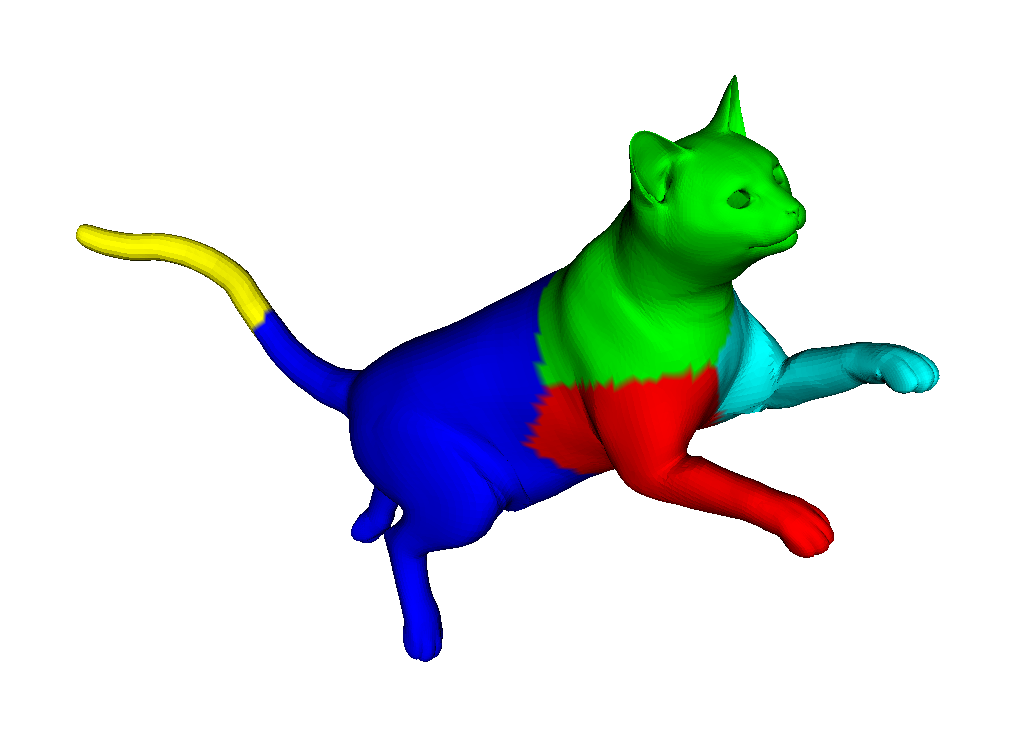
\includegraphics[width=\textwidth]{segmentation.png}}
				\only<2-2>{\includegraphics[width=\textwidth]<2>{rgb.png}}
				\only<3-3>{\includegraphics[width=\textwidth]<3>{scalar.png}}
			\end{figure}
      
    		\end{column}
  	\end{columns}
	
\end{frame}

\begin{frame}
	\frametitle{CustomTab}
	
	\begin{itemize}
		\item Constructor signature:
		\begin{itemize}
			\item \texttt{HashMap<vtkActor*, shared\_ptr<Shape>>\& \textcolor{blue}{shapes}}
			\item \texttt{HashMap<shared\_ptr<PointCorrespondence>, bool>\& \textcolor{blue}{pointCorrespondences}}
			\item \texttt{HashMap<shared\_ptr<FaceCorrespondence>, bool>\& \textcolor{blue}{faceCorrespondences}}
			\item \texttt{ShapeAnalyzerInterface* \textcolor{blue}{shapeAnalyzer}}
		\end{itemize}
		\item Abstract functions:
		\begin{itemize}
			\item \texttt{\textcolor{blue}{void} onShapeAdd(Shape* shape)}
			\item \texttt{\textcolor{blue}{void} onShapeEdit(Shape* shape)}
			\item \texttt{\textcolor{blue}{void} onShapeDelete(Shape* shape)}
			\item \texttt{\textcolor{blue}{void} onClear()}
		\end{itemize}
	\end{itemize}
\end{frame}

\begin{frame}[fragile]
\frametitle{Connect Custom Classes}

\lstset{language=C++,
                keywordstyle=\color{blue},
                stringstyle=\color{red},
                commentstyle=\color{green},
                morecomment=[l][\color{magenta}]{\#},
                numbers=none
}
\begin{lstlisting}
template<class T, class... Args>
class Factory { ... }

typedef Factory<CustomContextMenuItem, shared_ptr<Shape>, ShapeAnalyzerInterface*> CustomContextMenuItemFactory;

typedef Factory<CustomTab, const HashMap<vtkActor*, 
    shared_ptr<Shape>>&, 
    const HashMap<shared_ptr<PointCorrespondence>, bool>&, 
    const HashMap<shared_ptr<FaceCorrespondence>, bool>&, 
    ShapeAnalyzerInterface*> CustomTabFactory;
\end{lstlisting}

\end{frame}

\begin{frame}[fragile]
\frametitle{Connect Custom Classes}

\lstset{language=C++,
                keywordstyle=\color{blue},
                stringstyle=\color{red},
                commentstyle=\color{green},
                morecomment=[l][\color{magenta}]{\#},
                numbers=none
}
\begin{lstlisting}
struct CustomClassesRegistry {
    static void registerContextMenuItems() {
       CustomContextMenuItemFactory::getInstance()->Register<MyMenuItemClass>("key", "My Menu Item Label");
    }
    static void registerTabs() {
        CustomTabFactory::getInstance()->Register<MyTabClass>("key", "My Tab Label");
    }
}
\end{lstlisting}
  
\end{frame}


\begin{frame}[fragile]
\frametitle{Connect CustomContextMenuItems}
\lstset{language=C++,
                keywordstyle=\color{blue},
                stringstyle=\color{red},
                commentstyle=\color{green},
                morecomment=[l][\color{magenta}]{\#},
                numbers=none
}
\begin{lstlisting}
static void registerContextMenuItems() {
    CustomContextMenuItemFactory::getInstance()->Register<ExtractSegmentContextMenuItem>("extract_segment",
        "This>>is>>my>>menu path>>My item 1");
   
    CustomContextMenuItemFactory::getInstance()->Register<VoronoiCellsContextMenuItem<GeodesicMetric>>("voronoicells_geodesic",
        "This>>is>>My item 2");
}     
\end{lstlisting}
  \begin{figure}[h]
	\centering
	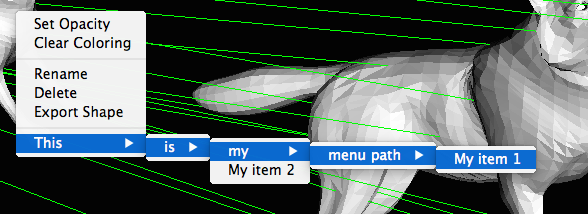
\includegraphics[width=0.60\textwidth]{menu.png}
\end{figure}
\end{frame}

\begin{frame}[fragile]
\frametitle{Connect CustomTabs}
\lstset{language=C++,
                keywordstyle=\color{blue},
                stringstyle=\color{red},
                commentstyle=\color{green},
                morecomment=[l][\color{magenta}]{\#},
                numbers=none
}
\begin{lstlisting}
static void registerTabs() {
    CustomTabFactory::getInstance()->Register<IdentityMatchingTab>("identity_matching", "Shapes>>My Shape Tab 1");

    CustomTabFactory::getInstance()->Register<ShapeInterpolationTab>("shape_interpolation", "Correspondences>>My Correspondences Tab 1");
}
\end{lstlisting}
  \begin{figure}[h]
	\centering
	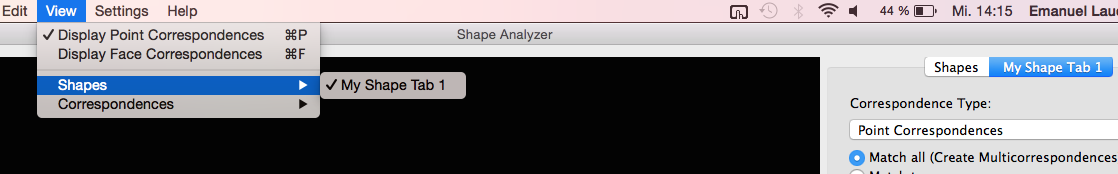
\includegraphics[width=\textwidth]{tabs.png}
\end{figure}
\end{frame}

\section{PETSc and SLEPc}
\begin{frame}
\frametitle{PETSc and SLEPc: A Linear algebra library}
\begin{itemize}
	\item PETSc: (Sparse) linear algebra (e.g. matrix vector multiplication, linear systems, ...)
	\item SLEPc: (Sparse) eigenvalue solver (builds up on PETSc)
	\item Heavily used in the "Computational Science and Engineering" community for solving PDEs (e.g. Computational Fluid Dynamics)
	\item Based on MPI (therefore well suited for distributed HPCs)
	\item Can also be used with CUDA and cuBLAS (instead of MPI).
	\item Drawback: Coding is kinda' low level :(
\end{itemize}
\end{frame}

\begin{frame}[fragile]
\frametitle{A Flavor of PETSc}
$$
	\mathbf{b} := \mathbf{A} \cdot \mathbf{a}
$$
\lstset{language=C++,
                keywordstyle=\color{blue},
                stringstyle=\color{red},
                commentstyle=\color{green},
                morecomment=[l][\color{magenta}]{\#},
                numbers=none
}
\begin{lstlisting}
    // Initialize matrix A
    int n = 10;
    int m = 15;
    Mat A;
    MatCreateSeqDense(PETSC_COMM_SELF, n, m, NULL, &A);
    for(PetscInt i = 0; i < n; i++) {
        for(PetscInt j = 0; j < m; j++) {
            PetscReal aij = rand();
            MatSetValue(A, i, j, aij, INSERT_VALUES);
        }
    }
    MatAssemblyBegin(A, MAT_FINAL_ASSEMBLY);
    MatAssemblyEnd(A, MAT_FINAL_ASSEMBLY);
\end{lstlisting}

\end{frame}

\begin{frame}[fragile]
\frametitle{A Flavor of PETSc}
$$
	\mathbf{b} := \mathbf{A} \cdot \mathbf{a}
$$
\lstset{language=C++,
                keywordstyle=\color{blue},
                stringstyle=\color{red},
                commentstyle=\color{green},
                morecomment=[l][\color{magenta}]{\#},
                numbers=none
}
\begin{lstlisting}
    //Initialization of the vectors a and b
    Vec a, b;
    MatGetVecs(A, &a, &b);
    for(PetscInt i = 0; i < size; i++) {
        VecSetValue(a, i, rand(), INSERT_VALUES);
    }
    VecAssemblyBegin(a);
    VecAssemblyEnd(a);
\end{lstlisting}

\end{frame}

\begin{frame}[fragile]
\frametitle{A Flavor of PETSc}
$$
	\mathbf{b} := \mathbf{A} \cdot \mathbf{a}
$$
\lstset{language=C++,
                keywordstyle=\color{blue},
                stringstyle=\color{red},
                commentstyle=\color{green},
                morecomment=[l][\color{magenta}]{\#},
                numbers=none
}
\begin{lstlisting}
    // Actual computation
    MatMult(A, a, b);
    VecView(b, PETSC_VIEWER_STDOUT_SELF);
    MatDestroy(&A);
    VecDestroy(&a);
    VecDestroy(&b);
\end{lstlisting}

\end{frame}

\begin{frame}[fragile]
\frametitle{A Flavor of PETSc and CUDA}
$$
	\mathbf{x} = a \cdot \mathbf{x} + \mathbf{y}
$$
\lstset{language=C++,
                keywordstyle=\color{blue},
                stringstyle=\color{red},
                commentstyle=\color{green},
                morecomment=[l][\color{magenta}]{\#},
                numbers=none
}
\begin{lstlisting}
ierr = VecCUDACopyToGPU(xin);CHKERRQ(ierr);
ierr = VecCUDACopyToGPU(yin);CHKERRQ(ierr);
try {
    cusp::blas::axpy(*((Vec_CUDA*)xin->spptr)->GPUarray,
        *((Vec_CUDA*)yin->spptr)->GPUarray,
        alpha
    );
    yin->valid_GPU_array = PETSC_CUDA_GPU;
    ierr = WaitForGPU();
    CHKERRCUDA(ierr);
} catch(char *ex) { /*...*/ }
\end{lstlisting}

\end{frame}

\section{A Function Transfer Tab}
\begin{frame}[fragile]
\frametitle{A Function Transfer Tab}
\bf{Demo time}
\end{frame}

\begin{frame}
\frametitle{Functional maps: Intro}
Goal: Transfer a function $f_M:V_M \to \mathbb{R}$ from shape $M$ to shape $N$. (Note: $M = (V_M:=\{v_1, v_2, \dots, v_n\}, T_M)$ and therefore $f \in \mathbb{R}^n$)\\
Assumption: $M$ and $N$ are related by an \emph{isometry}
\end{frame}

\begin{frame}[fragile]
\frametitle{Functional maps: ONB}
$$
	f = \sum_{i=1}^{n} a_i\phi_i \in \mathbb{R}^n
$$
First guess (Canonical basis of $\mathbb{R}^n$): $\phi_i := \delta_{ij}$ \\

\begin{block}{}
Q: Is this really a good idea? A: Nope!
\begin{itemize}
	\item Both shapes are required to have same number of vertices ($m=n$)
	\item Transferring a function $f$ from $M$ to $N$ requires correspondence Matrix $C\in \mathbb{R}^{n \times n}$ (But that is what we are looking for)
\end{itemize}
\end{block}
\end{frame}

\begin{frame}[fragile]
\frametitle{Functional maps: ONB}
Better choice:
Eigenvectors $\{\phi^M_i\}_{i=1}^n \subset \mathbb{R}^n$ and $\{\phi^N_i\}_{i=1}^m \subset \mathbb{R}^m$ of the Laplace-Beltrami operators $\Delta_M=M_M^{-1} \cdot L_M \in \mathbb{R}^{n \times n}$ and $\Delta_N=M_N^{-1} \cdot L_N \in \mathbb{R}^{m \times m}$
\begin{figure}[h]
	\centering
	\includegraphics[width=1.0\textwidth]{Michael.eps}
\end{figure}
  \begin{figure}[h]
	\centering
	\includegraphics[width=1.0\textwidth]{Michael1.eps}
\end{figure}

\end{frame}

\begin{frame}[fragile]
\frametitle{Functional maps: ONB}
\begin{block}{Property}
If two shapes $M, N$ are related by a perfect isometry, their Laplace-Beltrami eigenvectors are the same up two sign flip.
\end{block}
\begin{block}{Idea}
Transfer $f$ from $M$ to $N$ by projecting it onto Laplace-Beltrami eigenbasis $\{\phi_i\}_{i=1}^{20}$ and flip signs of coefficients accordingly:
$$
	 \langle \phi_i^M, f \rangle = \langle \phi_i^M, \sum_{j=1}^{20} a_j\phi_j^M \rangle = \sum_{j=1}^{20} a_j \langle \phi_i^M, \phi_j^M  \rangle = a_i 
$$
$$
	t(f) = \sum_{i=1}^{20} b_i \phi_i^N = \sum_{i=1}^{20} c_{ii} a_i \phi_i^N \quad \text{with } c_{ii} \in \{-1, 1\} 
$$
\end{block}
\end{frame}

\begin{frame}[fragile]
\frametitle{Functional maps: Idea}
$$
	t(f) = \sum_{i=1}^{20} c_{ii} a_i \phi_i^N = \underbrace{C \cdot a}_{=b} \cdot \Phi^N \quad \text{with } C \in \mathbb{R}^{20 \times 20}, C \text{ diagonal} 
$$
Since we never deal with perfect isometries $C$ is not perfectly diagonal:
\begin{figure}[h]
	\centering
	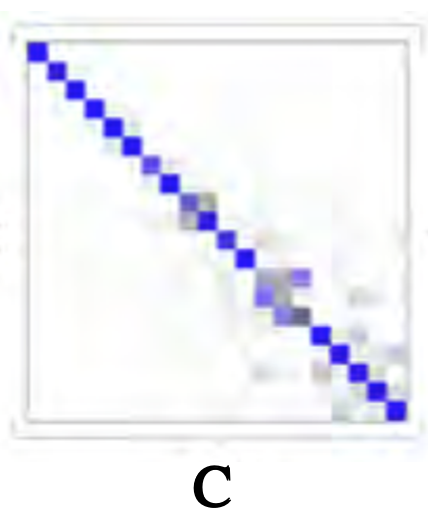
\includegraphics[width=.3\textwidth]{C.png}
\end{figure}
\end{frame}

\begin{frame}[fragile]
\frametitle{Functional maps: Compute C}
Assume we are given a set of corresponding constraint functions represented as 20-dimensional vectors of coefficients $a_i^\top,b_i^\top \in \mathbb{R}^{20}$:
$$
	\min_C \frac{1}{2} \| B - CA \|_F^2 + \lambda |W \circ C|_1
$$
\end{frame}
\begin{frame}[fragile]
\frametitle{Functional maps: Define W}
First guess: Squared distance from diagonal: $C_{ij}:=10 \cdot (i-j)^2$\\
Better:
$$
	C_{ij} :=\min\{|i - j|, 1\} \cdot (100 - \left(\frac{\min\{i, j\}}{20}\right)^3 \cdot 100)
$$
\begin{figure}[htp]
  \begin{center}
    \subfigure{
\includegraphics[scale=0.15]{W_1.eps}}
    \subfigure{
\includegraphics[scale=0.15]{W_2.eps}} 
    \subfigure{
\includegraphics[scale=0.15]{W_3.eps}}
  \end{center}
\end{figure}
\end{frame}

\begin{frame}[fragile]
\frametitle{Functional maps: Outliers}
$$
	\min_{C,O} \frac{1}{2} \| B - CA -O \|_F^2 + \lambda |W \circ C|_1 + \mu \|O\|_{2,1}
$$
where $\|O\|_{2,1}:= \sum_{i=1}^l \|o_i^\top \|_2$
\end{frame}

\section*{}

\begin{frame}
\frametitle{Questions?}
\bf{Thank you for your attention!}
\end{frame}

\end{document}
